\documentclass[12pt,a4paper]{report}

    \newcommand{\varTitle}{Geotechnical Simulations with Moose}
    \newcommand{\varAuthor}{Jörg Meier}
    \newcommand{\varDate}{27.01.2025}

    % General document formatting
    \usepackage[margin=0.7in]{geometry}
    \usepackage[parfill]{parskip}
    \usepackage[utf8]{inputenc}
    \usepackage[]{mdframed}
    \usepackage{tikz}
    \usetikzlibrary{shapes.geometric, arrows, arrows.meta, chains, positioning}
    \usepackage{graphicx}
    \usepackage[edges]{forest}
    \usetikzlibrary{decorations.pathreplacing}

    % tables
    \usepackage{tabularx,array,booktabs,multirow}
    \newcolumntype{Y}{>{\centering\arraybackslash}X} % for centering tables in tabularx
    \usepackage{makecell}

    % Related to math
    \usepackage{amsmath,amssymb,amsfonts,amsthm}

    % make links clickable
    \usepackage{hyperref}
    \hypersetup{
        colorlinks    = true,    % Colours links instead of ugly boxes
        urlcolor      = blue,    % Colour for external hyperlinks
        linkcolor     = black,   % Colour of internal links
        bookmarksopen = true,
        citecolor     = black     % Colour of citations
    }
    \usepackage[nameinlink,noabbrev]{cleveref}

    \newcommand*{\shortautoref}[1]{%
        \begingroup
        \def\sectionautorefname{sec.}%
        \def\subsectionautorefname{sec.}%
        \autoref{#1}%
        \endgroup
    }

    \newcommand{\light}[1]{\textcolor{gray}{#1}}

    % Other packages
    \usepackage[inline]{enumitem}
    \usepackage{soul}   %for highlighting text
    % \usepackage{layouts}
    \usepackage{fontawesome5}

    % captions
    \usepackage{caption}
    \captionsetup{justification=raggedright,singlelinecheck=false}
    \usepackage{subcaption}

    % colors
    \usepackage{xcolor}
    \definecolor{dkgreen}{rgb}{0,0.6,0}
    \definecolor{gray}{rgb}{0.5,0.5,0.5}
    \definecolor{mauve}{rgb}{0.58,0,0.82}

    % code listings
    \usepackage{listings}
    \usepackage{textcomp} % for for straight single quotes (upquote=true)
    \lstdefinelanguage{Moose}{
        sensitive=f,%
        morecomment=[l]{\#},% comments
        morekeywords={true,false},%
        morestring=[b]{"},% strings with double quote
        morestring=[b]{'},% strings with single quote
        upquote=true, % for straight single quotes (see https://tex.stackexchange.com/questions/145416/how-to-have-straight-single-quotes-in-lstlistings)
        morecomment=[s][\color{blue}\ttfamily]{\[}{\]},% block names and block endings
        morecomment=[s][\color{BlueViolet}\ttfamily]{\$\{}{\}},% references to variables etc. ${...}
        literate= %{=}{{\color{blue}= }}1
                 {á}{{\'a}}1 {é}{{\'e}}1 {í}{{\'i}}1 {ó}{{\'o}}1 {ú}{{\'u}}1
                 {Á}{{\'A}}1 {É}{{\'E}}1 {Í}{{\'I}}1 {Ó}{{\'O}}1 {Ú}{{\'U}}1
                 {à}{{\`a}}1 {è}{{\`e}}1 {ì}{{\`i}}1 {ò}{{\`o}}1 {ù}{{\`u}}1
                 {À}{{\`A}}1 {È}{{\`E}}1 {Ì}{{\`I}}1 {Ò}{{\`O}}1 {Ù}{{\`U}}1
                 {ä}{{\"a}}1 {ë}{{\"e}}1 {ï}{{\"i}}1 {ö}{{\"o}}1 {ü}{{\"u}}1
                 {Ä}{{\"A}}1 {Ë}{{\"E}}1 {Ï}{{\"I}}1 {Ö}{{\"O}}1 {Ü}{{\"U}}1
                 {â}{{\^a}}1 {ê}{{\^e}}1 {î}{{\^i}}1 {ô}{{\^o}}1 {û}{{\^u}}1
                 {Â}{{\^A}}1 {Ê}{{\^E}}1 {Î}{{\^I}}1 {Ô}{{\^O}}1 {Û}{{\^U}}1
                 {ã}{{\~a}}1 {ẽ}{{\~e}}1 {ĩ}{{\~i}}1 {õ}{{\~o}}1 {ũ}{{\~u}}1
                 {Ã}{{\~A}}1 {Ẽ}{{\~E}}1 {Ĩ}{{\~I}}1 {Õ}{{\~O}}1 {Ũ}{{\~U}}1
                 {œ}{{\oe}}1 {Œ}{{\OE}}1 {æ}{{\ae}}1 {Æ}{{\AE}}1 {ß}{{\ss}}1
                 {ű}{{\H{u}}}1 {Ű}{{\H{U}}}1 {ő}{{\H{o}}}1 {Ő}{{\H{O}}}1
                 {ç}{{\c c}}1 {Ç}{{\c C}}1 {ø}{{\o}}1 {Ø}{{\O}}1 {å}{{\r a}}1 {Å}{{\r A}}1
                 {€}{{\euro}}1 {£}{{\pounds}}1 {«}{{\guillemotleft}}1
                 {»}{{\guillemotright}}1 {ñ}{{\~n}}1 {Ñ}{{\~N}}1 {¿}{{?`}}1 {¡}{{!`}}1 ,%
        alsoletter={=!},%
        morekeywords=[2]{=,!include},%
        keywordstyle=[2]{\color{blue}},%
        %https://tex.stackexchange.com/questions/217505/listings-color-numbers-only-out-of-keywords
    }[keywords,comments,strings]

    \lstset{frame=tb,
        language=Moose,
        aboveskip=3mm,
        belowskip=3mm,
        showstringspaces=false,
        columns=flexible,
        basicstyle={\small\ttfamily},
        numbers=none,
        numberstyle=\tiny\color{gray},
        keywordstyle=\color{blue},
        commentstyle=\color{dkgreen},
        stringstyle=\color{mauve},
        breaklines=true,
        breakatwhitespace=true,
        tabsize=3,
        % deletekeywords={from,in,and},
        % morekeywords={function,Algorithm,algorithm, then,do},
    }

    % awesomebox
    \usepackage{awesomebox}

    % todo
    \setlength {\marginparwidth }{2cm}
    \usepackage{xargs}                      % Use more than one optional parameter in a new commands
    \usepackage[dvipsnames]{xcolor}  % Coloured text etc.
    \usepackage[colorinlistoftodos,prependcaption,textsize=tiny]{todonotes}
    \newcommandx{\unsure}[2][1=]{\todo[linecolor=red,backgroundcolor=red!25,bordercolor=red,#1]{#2}}
    \newcommandx{\change}[2][1=]{\todo[linecolor=blue,backgroundcolor=blue!25,bordercolor=blue,#1]{#2}}
    \newcommandx{\info}[2][1=]{\todo[linecolor=OliveGreen,backgroundcolor=OliveGreen!25,bordercolor=OliveGreen,#1]{#2}}
    \newcommandx{\improvement}[2][1=]{\todo[linecolor=Plum,backgroundcolor=Plum!25,bordercolor=Plum,#1]{#2}}
    \newcommandx{\thiswillnotshow}[2][1=]{\todo[disable,#1]{#2}}
    \newcommandx{\todoinline}[2][1=]{
        {\hbadness=10000 \hfuzz=\maxdimen{\todo[inline,linecolor=Plum,backgroundcolor=Plum!25,bordercolor=Plum,#1]{#2}}}
        % \errmessage{#2}
        % \GenericError{9}{#2}{0}{1}
        % \GenericInfo{9}{#2}
        % \PackageWarning{ToDo}{#2}
        % \typeout{Package ToDo Warning: #2}\typeout{}
        % \typeout{Package ToDo Info: #2}\typeout{}
    }

    \NewDocumentCommand{\codeword}{v}{%
        \texttt{\textcolor{blue}{#1}}%
    }

    % Bulleted command: insert a sing bulleted item without any margins
    \newcommandx{\bulleted}[1]{%
        \begin{minipage}[t]{\linewidth}
            \begin{itemize}[nosep, leftmargin=1em, labelwidth=*,align=left]
                \item #1
            \end{itemize}
        \end{minipage}
    }

    \usepackage{filemod}

    \tikzstyle{startstop} = [rectangle, rounded corners, minimum width=3cm,
    minimum height=1cm, text centered, draw=black]
    \tikzstyle{process} = [rectangle, minimum width=3cm,
    minimum height=1cm, text centered, draw=black]
    \tikzstyle{decision} = [diamond, minimum width=3cm,
    minimum height=1cm, text centered, draw=black]
    \tikzstyle{arrow} = [thick, ->, >=stealth]

    % physial units
    \usepackage{siunitx}
    \DeclareSIUnit\year{a}
    \DeclareSIUnit\metreabovesealevel{\text{m ü.M.}}
    \DeclareSIUnit\ton{\text{t}}
    \DeclareSIUnit\DOF{\text{DOF}}

    % attach files
    \usepackage{currfile}
    \usepackage{attachfile}

    \newcommandx{\fileattachment}[2]{\textattachfile[color=0 0 0]{#1}{\faFile*[regular] #2}}

    % comments
    % \usepackage[opacity=0]{pdfcomment}
    % {\pdftooltip[style = mathpopup]{ \mu_\mathrm{f} }{ dynamic viscosity of the fluid }}

\title{\varTitle}

\author{\varAuthor}

\date{\varDate}

% References
\usepackage[square,sort,comma,numbers,sectionbib]{natbib}
\usepackage{multibib}
\newcites{Publications}{Publications}
% \newcites{Standards}{Standards and Recommendations}

\begin{document}

% awesomebox: override default box with to avoid overfull \hbox warning
\setlength{\aweboxcontentwidth}{0.81\linewidth}

\lstset{language=[Sharp]C,,basicstyle=\footnotesize\ttfamily,showspaces=false,showtabs=false,,breaklines=true,showstringspaces=false,breakatwhitespace=true, escapeinside={(*@}{@*)}}

%\maketitle
\begin{titlepage}
    \begin{flushright}
        \includegraphics[width=4.5cm]{img/gruner.pdf}
    \end{flushright}
    \begin{center}
        \vspace*{5cm}

        {\Huge\textbf{Geotechnical Simulations with Moose}}

        \vspace{5cm}
        %Upgrade Report

        \large{-- DRAFT --}

        \vfill

        \large{This whitepaper collects information and code \\
            for geotechnical simulations with the software Moose.}

        \vfill

        \textbf{Jörg Meier}

        \vspace{0.8cm}

        Gruner AG, Geotechnical Engineering\\
        Basel, Switzerland\\

        \vspace{1cm}
        16.10.2024\\

        \vspace{1cm}
        License: CC-BY-SA-4.0

    \end{center}
\end{titlepage}

\tableofcontents

\chapter{Introduction}
\label{chap:introduction}
The open-source, parallel finite element framework Moose
(\url{mooseframework.inl.gov}) can also be used to perform simulations that are
used in the geotechnical design practice. This document aims to collect options
and techniques that are suitable for creating such geotechnical simulations
with Moose.

In the geotechnical planning practice, finite element models are often used for
deformation prognosis. Furthermore, such FE models can help to identify complex
failure mechanisms. The requirements for these models are accordingly a
sufficiently good representation of the geotechnical structure including the
subsoil, the groundwater conditions, pre-existing structures and similar. These
FE models simulate the construction process over time. As this design process
is generally intended to take place in a controlled and quasi-static form, the
associated simulations are usually also transient and quasi-static. Therefore,
scope and main focus of this document are transient quasi-static simulations.

This document is primarily intended as a collection of information rather than
a textbook or step-by-step guide. As such, it is intended to be a 'living'
document that will be continually edited and updated.

This document is published under the
\href{https://creativecommons.org/licenses/by-sa/4.0/}{CC-BY-SA-4.0} license.
No warranties are given.

\chapter{General Remarks}
\label{chap:general}
\section{Sign convention}
\label{chap:sign-convention}

% https://github.com/idaholab/moose/discussions/20999
% https://github.com/idaholab/moose/discussions/29182#discussioncomment-11456527

In the [SolidMechanics] module and the [PorousFlow] module the sign convention
is as follows:

\begin{itemize}
      \item Positive strain is extensional, which (usually) results from a positive
            (tensile) stress.
      \item Negative strain is compressional, which (usually) results from a negative
            (compressive) stress.
      \item Compressive pore-pressures (e.g. below a free water table) have a positive
            sign.
      \item Suction is represented by pore-pressures having a negative sign.
\end{itemize}


\chapter{Model Configuration}
\label{chap:setup}
\section{Strain calculation}
\label{chap:model-configuration-strain}

In the
\href{https://mooseframework.inl.gov/modules/solid_mechanics/}{'solid\_mechanics'}
module, Moose supports three different types of
\href{https://mooseframework.inl.gov/modules/solid_mechanics/Strains.html}{strain}
calculation:
\begin{itemize}
  \item {Small Linearized Total Strain}
  \item {Incremental Small Strains}
  \item {Finite Large Strains}
\end{itemize}

\begin{lstlisting}[language=perl, caption={Setting up incremental small strains within the Physics/SolidMechanics block},label={setup-incremental-small-strains}]
[Physics]
  [SolidMechanics]
    [QuasiStatic]
      [./all]
        strain = SMALL
        incremental = true
        (*@{\raisebox{-1pt}[0pt][0pt]{$\vdots$}}@*)
      []
    []
  []
[]
\end{lstlisting}

\section{Stress calculation}
\label{chap:model-configuration-stress}

\href{https://mooseframework.inl.gov/modules/solid_mechanics/Stresses.html}{Stresses.html}

The stress calculation chosen by the user must be compatible with the strain
calculation (\autoref{chap:model-configuration-strain}).

ComputeFiniteStrainElasticStress for incremental and finite strain
formulations.

(to be written)

\chapter{Geometry}
\label{chap:geometry}
\section{General Considerations}
\label{geometry-general}

When modelling geotechnical problems, it is often desirable to
make a meaningful geometric abstraction to avoid time-consuming
modelling, but also to avoid inaccuracies due to oversimplification.
However, experience shows that the effort involved in creating such
a model geometry should not be underestimated and that the models
consist of a large number of individual parts and components.
Some of these objects have trivial shapes (e.g. rectangular surfaces
for a sheet pile wall segment), others can have non-trivial curvilinear
boundaries (e.g. geological bodies).
All of these objects must be shaped to fit each other (without gaps or
overlaps) and together form the FE model.

As the shape of these individual parts and components directly influences
the shape of the FE elements they are build of, further prerequisites must
be considered during geometrisation: For instance, as few ‘unfavourably
shaped’ (e.g. too acute-angled) FE elements as possible should result in
order to avoid numerical instabilities or load increments that are too
small. A common reason for acute-angled elements and large numbers of
elements are corner or end points that are close together and unfavourable
intersections of the objects. Another requirement for geometrisation
is that the number of FE elements should remain within a range that
enables acceptable calculation times.

Although Moose's ‘Mesh System’ provides a variety of tools for generating
FE meshes on the basis of input file commands, the creation of geometrically
complex models with these commands is often confusing and error-prone.
% https://mooseframework.inl.gov/syntax/Mesh/index.html

The mesh is therefore often created outside of the Mosse (e.g. using
\href{https://blender.org}{Blender}), saved as MSH-file and then imported
using the \codeword{FileMeshGenerator}.
The code required for this import in a Moose input file is shown in
listing \ref{FileMeshGenerator}.
% \href{https://mooseframework.inl.gov/source/meshgenerators/FileMeshGenerator.html}{FileMeshGenerator}

\begin{lstlisting}[caption={Read mesh from a file},label={FileMeshGenerator}]
[Mesh]
    [file]
        type = FileMeshGenerator
        file = "source.msh"
    []
    second_order = true
[]
\end{lstlisting}

(to be written)


\chapter{Modelling of geometric entities, structures, loads, etc.}
\label{chap:entities}
This chapter collects information on how different types of geometric entities,
structures, loads etc. can be modelled.

(to be written)

\section{Overview}

\begin{table}
    \begin{tabularx}{\textwidth}{@{}lXl@{}}
        \hline
        Entity
         &
        Options for Modelling
         &
        Reference
        \\

        \hline
        soil volume
         &
        \bulleted{cluster of volume elements}
         &
        \autoref{chap:entities-volume}
        \\

        \hline
        excavation pit wall
         &
        \bulleted{shell elements}
         &
        \autoref{chap:entities-shell}
        \\

         &
        \bulleted{cluster of volume elements in case of a 'thick' wall (e.g. slurry wall, bored pile wall)}
         &
        \autoref{chap:entities-volume}
        \\

        \hline
        pile
         &
        \bulleted{cluster of volume elements in case of a pile with large diameter (e.g. bored pile)}
         &
        \autoref{chap:entities-volume}
        \\

        %  &
        % \bulleted{embedded beams}
        %  &
        % \autoref{chap:entities-embedded-beams}
        % \\

        \hline
        prop
         &
        \bulleted{spring between nodes}
         &
        \autoref{chap:entities-springs}
        \\

         &
        \bulleted{fixed end spring}
         &
        \autoref{chap:entities-fixed-end-springs}
        \\

         &
        \bulleted{beam}

         &
        \autoref{chap:entities-beams}
        \\

        \hline
    \end{tabularx}
    \caption{Selected geotechnical entities and their respective modelling}
    \label{tab:myfirsttable}
\end{table}

\section{Entities}
% \label{chap:entities}

\subsection{Volumes}
\label{chap:entities-volume}

\subsection{FixedEndSprings}
\label{chap:entities-fixed-end-springs}

https://mooseframework.inl.gov/source/nodalkernels/CoupledForceNodalKernel.html

https://onlinelibrary.wiley.com/doi/pdf/10.1002/pamm.202200045

\subsection{Springs between nodes (NodeToNodeAnchors)}
\label{chap:entities-springs}

https://mooseframework.inl.gov/mastodon/source/materials/LinearSpring.html

\subsection{Beams (line element)}
\label{chap:entities-beams}

% \subsection{EmbeddedBeams (line element)}
% \label{chap:entities-embedded-beams}

\subsection{Shell (surface element)}
\label{chap:entities-shell}

\subsection{Interfaces (surface element)}

\subsection{Contact}

\subsection{Pore Pressure Boundaries}


\chapter{Initial Conditions}
\label{chap:initial}
\section{Initial conditions for Moose objects}
\label{chap:IC-moose-objects}

For definition of the initial (starting) conditions for the variables a Moose
simulation the \href{https://mooseframework.inl.gov/syntax/ICs}{ICs system} is
to be used.

(to be written)

\section{Gravitation and initial stress state}
\label{chap:IC-stress-state}

The initial stress state of geotechnical simulations is often non-trivial. This
is because the section of geosphere to be modelled often has a history of
millions of years under different loading conditions, including gravity and
tectonic processes. In addition, the Earth's surface is often non-horizontal,
so that stress trajectories near the surface are oriented accordingly.
Furthermore, the initial stress state may be anisotropic with a specific
orientation. Gravity and the initial stress state are normally taken into
account by a combination of the following elements:

\begin{itemize}
  \item Definition of appropriate displacement boundary conditions for the model (see
        \autoref{chap:model-configuration-boundary-fixities}).
  \item Activation of gravitational body force (see
        \autoref{chap:IC-stress-state-gravity}).
  \item Definition of eigenstrains from the initial stress field (e.g. using
        \href{https://mooseframework.inl.gov/source/materials/ComputeEigenstrainFromInitialStress.html}{ComputeEigenstrainFromInitialStress},
        see \autoref{chap:IC-stress-state-simple} and
        \autoref{chap:IC-stress-state-anisotropic}).
\end{itemize}

\importantbox{
  In simulations including pore water, ‘effectice stresses’ are to be used.
  This includes the definition of the initial stress field, where also
  effective stresses are to be given.
}

\subsection{Gravity}
\label{chap:IC-stress-state-gravity}

To consider gravity, the following aspects must be included in the model:
\begin{itemize}
  \item When compiling the MooseApp: As the effect of gravity is taken into account in
        interaction with the material density, the Moose module \codeword{MISC} must be
        active in addition to the Moose module \codeword{SOLID_MECHANICS}.
  \item Gravity must be activated in the input file. This is done by adding a special
        kernel of the type \codeword{Gravity} as shown in
        \autoref{initial-conditions-gravity}. The direction and strength of the
        gravitational field is to be defined here.
  \item The materials must be assigned a material density
        (\autoref{initial-conditions-density}).
\end{itemize}

\begin{lstlisting}[language=perl, float, caption={Gravity kernel in a Moose inut file},label={initial-conditions-gravity}]
[Kernels]
    [gravity]
        type = Gravity
        use_displaced_mesh = false
        variable = disp_z           # the displacement variable the gravity is associated with
        value = -9.81               # in m/s^2
    []
[]
\end{lstlisting}

\begin{lstlisting}[language=perl, float, caption={Assignment of a density to subdomain ‘block1’},label={initial-conditions-density}]
[Materials]
    [undrained_density]
      type = GenericConstantMaterial
      block = 'Block1'
      prop_names = density
      prop_values = 2500            # in kg/m^3
    []
[]
\end{lstlisting}

{\hfuzz=20pt
\subsection{Initial stress state using ComputeEigenstrainFromInitialStress}
}
\label{chap:IC-stress-state-simple}

In a uninfluenced homogeneous horizontal half-space (or a section thereof)
under the effect of gravity, the initial stress state corresponds to a
‘geostatic stress field’. This geostatic stress field can be represented
analytically for a stress point as follows:

\begin{equation}
  \sigma'_{ini,vert}=\sigma'_{ini,vert,h=0}+\gamma' h
\end{equation}
\begin{equation}
  \sigma'_{ini,horiz}=\sigma'_{ini,vert} K_0 \quad \text{with } \quad K_0 = 1-\sin\varphi
\end{equation}

In these equations, $\gamma'=\rho' g$ corresponds to the weight of the soil,
$h$ to the overburden height, $\sigma'_{ini,vert,h=0}$ to the effective
vertical stress at $h=0$ and $K_0$ to the earth pressure coefficient. This
earth pressure coefficient is usually estimated as a function of the angle of
internal friction $\varphi$ (simplified equation according to Jaky).

\autoref{initial-conditions-ComputeEigenstrainFromInitialStress} shows the
definition of a geostatic initial stress state using two functions
\codeword{ini_xx_yy} and \codeword{ini_zz} and their subsequent use in a
\codeword{ComputeEigenstrainFromInitialStress}.

\begin{lstlisting}[language=perl, float, caption={Definition of a geostatic initial stress state using ‘ComputeEigenstrainFromInitialStress’ },label={initial-conditions-ComputeEigenstrainFromInitialStress}]
[Functions]
    [ini_xx_yy]   # function describing the initial effective horizontal stress field
      type = ParsedFunction
      vars = 'sig_top   z_top   rho      g    k0 '
      vals = '-1.5      0       0.0025   10   0.3'
      value = '(sig_top - rho * g * (z_top - z)) * k0'
    []
    [ini_zz]      # function describing the initial effective vertical stress field
      type = ParsedFunction
      vars = 'sig_top   z_top   rho      g'
      vals = '-1.5      0       0.0025   10'
      value = '(sig_top - rho * g * (z_top - z))'
    []
[]
  
[Materials]
    [strain]
      type = ComputeIncrementalSmallStrain
      volumetric_locking_correction = false
      eigenstrain_names = ini_stress        # pointing to the initial stress field
    []
    [ini_stress]   # initial stress field (effective stresses)
      type = ComputeEigenstrainFromInitialStress
      eigenstrain_name = ini_stress
      initial_stress = 'ini_xx_yy 0 0   0 ini_xx_yy 0   0 0 ini_zz'
    []
[]
\end{lstlisting}

\subsection{Initial stress state for anisotropic stresses}
\label{chap:IC-stress-state-anisotropic}

Align the model to the orientation of the initial stresses

(to be written)

\subsection{Checking the initial stress state}
\label{chap:IC-check}

In geotechnics, the initial state including the initial stress state should be
in equilibrium. Therefore, in a first time step without any changes to the
model ‘nothing’ should happen (only neglectable deformations and changes in the
stress field).

This can be checked by introducing such a time step without any changes as a
first time step and assessing the system response (e.g. in Paraview).


\chapter{Construction Stages}
\label{chap:stages}
\section{General comments on construction stages}
\label{chap:stages-general}

The type of geotechnical simulation primarily discussed in this document aims
to model a construction process. Accordingly, such a simulation must reproduce
the various stages of construction over time. Since this document assumes that
Moose models are organised on the basis of subdomains
(\autoref{geometry-blocks-and-subdomains}), the state changes also refer
primarily to adjustments that affect entire subdomains.

The most common state changes in this context are:

\begin{itemize}
      \item Activating FE-elements (e.g. installation of sheet piles is usually modelled by
            activating the corresponding set ot FE-elements,
            \autoref{chap:stages-element-activation-deactivation})
      \item Deactivating FE-elements (e.g. excavation of a soil volume is usually modelled
            by deactivating the corresponding set of FE-elements,
            \autoref{chap:stages-element-activation-deactivation})
      \item Replacing FE-elements (e.g. installation of a slurry wall modelled via volume
            elements leads to the need to replace the soil volume with the volume
            representing the slurry wall, \autoref{chap:stages-element-replacement})
      \item Adjusting external loads (e.g. loads are used to model various influences. As
            these influences change over time, the corresponding loads have to be adjusted,
            \autoref{chap:stages-loads})
      \item Adjusting prestress (e.g. for props and stand anchors the prestress is to be
            adjusted, \autoref{chap:stages-prestress})
\end{itemize}

As a consequence of the Moose input file concept, these status adjustments must
be triggered at various points in an input file if Moose is used ‘out of the
box’. To provide a more centralised way of defining construction stages, the
\codeword{[Stages]} MooseApp code plugin linked below can be used:

\href{https://github.com/jmeier/moose-codeplugin-stages}{github.com/jmeier/moose-codeplugin-stages}

This document primarily describes the procedure for the definition of
construction stages, with the use of the \codeword{[Stages]} code plugin where
applicable. The procedure without this plugin is only mentioned in selected
places.

\section{Time steps without changes}
\label{chap:stages-without-changes}

Avoid time steps (and therefore stages) without changes to the model. Time
steps without changes may not converge, even if a convergence was found for the
previous time step - compared to which no changes were made (due to the
relative error being ‘high’).

\todoinline{elaborate on timesteps without changes}

\section{Abrupt versus gradual changes}
\label{chap:stages-gradual-changes}

For transient simulations, the speed at which changes are applied to the model
is usually important. When elements are deactivated, the self-weight of these
elements is removed, all loads and stresses transmitted by these elements must
be redistributed, and so on. If many elements are deactivated, the resulting
changes in the stress field will be correspondingly large. In a not purely
linear-elastic model, comprehensive changes can lead to numerical instability,
resulting in slow or no convergence.

For geotechnical problems, on the other hand, changes in reality are usually
gradual.

(to be written)

\section{Activating and deactivating FE-elements}
\label{chap:stages-element-activation-deactivation}

%check: https://caeassistant.com/blog/abaqus-element-deletion-criteria/

As mentioned in \autoref{geometry-blocks-and-subdomains}, Moose models are
organized and managed by means of subdomains. By assigning FE elements and
materials to a subdomain, for example, the behaviour of these FE elements is
defined. However, Moose does not offer the option of activating or deactivating
FE elements or subdomains during a simulation run. However, Moose allows FE
elements to be reassigned from one subdomain to another during a simulation run
using the
\href{https://mooseframework.inl.gov/syntax/MeshModifiers/index.html}{MeshModifiers}
system.

On the other hand, Moose allows for subdomains to exist without kernels,
variables, materials and other Moose objects, but for FE elements to be present
in these subdomains. FE-elements in those subdomains ‘without physics’ will
simply be ignored my Moose.

Activation and deactivation of FE elements can thus be modelled by combining
the option to have subdomains ‘without physics’ and the option to reassign FE
elements to another subdomain. For deactivation FE elements are moved from a
subdomain ‘with physics’ to a subdomain ‘without physics’. For activation vice
versa.

ToDo:
\begin{itemize}
      \item Activation / Deactivation with [Stages]
      \item Ramp up / ramp down material properties, \autoref{chap:stages-gradual-changes}
\end{itemize}

\section{\todomarker Replacing FE-elements}
\label{chap:stages-element-replacement}

(to be written)

\section{\todomarker Adjusting external loads}
\label{chap:stages-loads}

(to be written)

\section{\todomarker Adjusting prestress}
\label{chap:stages-prestress}

(to be written)

\chapter{Material Models for Soil and Rock}
\label{chap:materials}
\section{Preliminary remarks on the material models}
\label{chap:material-remarks}

The built-in library of material models suitable for modelling soil and rock is
currently very limited.

\section{NEML2}
\label{chap:material-NEML2}

Moose supports the use of materials defined by means of the external material
modeling library \href{https://github.com/reverendbedford/neml2}{NEML2}
(Messner and Hu). Details on the integration of NEML2 into Moose are not scope
of this document and can be found in the corresponding
\href{https://mooseframework.inl.gov/moose/modules/solid_mechanics/NEML2.html}{corresponding
    section of the Moose documentation}.

\section{Mohr-Coulomb (linear-elastic ideal-plastic)}
\label{chap:material-mohr-coulomb}

(to be written)


\chapter{Proven Patterns}
\label{chap:patterns}
\section{Partial input files}
\label{chap:patterns-partial-input-files}

When a Moose model is defined as an
\href{https://mooseframework.inl.gov/application_usage/input_syntax.html}{‘input
    file’} (usually with the file extension ‘*.i’), the size of such an input file
can quickly grow to several hundred lines, even without the model geometry.
Editing and troubleshooting becomes correspondingly confusing. Moose therefore
also supports ‘partial input files’, where other input files can be called up
from a ‘central’ input file. For example, the material parameters or variables
with groups of geometrical objects could be maintained in a separate file.

The recommented option is to use the \codeword{!include} keyword within the
input file. This option is shown in \autoref{patterns-include}. Please note,
that the neither path not filename are allowed to contain a newline character,
\codeword{#} character, or \codeword{[} character.

\begin{lstlisting}[language=perl, caption={Include anpther input file},label={patterns-include}]
!include "path/to/file.i"
\end{lstlisting}

The alternative and not recommented option is to call a Moose app with several
input files as arguments. These input files are interpreted by simply
concatenating them. This functionality was included in Moose for test purposes,
but is not suitable for productive models, as this call may not be not
documented and may not be reproducible:

\codeword{./moose-opt -i input1.i -i input2.i -i input3.i}

\section{Physical units}
\label{chap:patterns-physical-units}

(to be written)

\begin{lstlisting}[language=perl, caption={Physical units in inut files},label={patterns-physical-units}]
    E = ${units 1000E3 kN/m^2 -> MN/m^2}

    # variable holding the pyhsical unit for lengths
    modelunit_length = 'm'
    
    # Umrechnung von 10 mm in die Modelleinheit (m)
    a = ${units 10 mm -> ${modelunit_length}}


    # model units
    modelunit_length = 'm'
    modelunit_time   = 's'
    modelunit_mass = 'kg' # Mg = tons; Gg = kilotons

    # derived units (this may be moved into a !include)
    modelunit_force  = ${raw ${modelunit_mass} * ${modelunit_length} / ${modelunit_time} ^ 2}
    modelunit_pressure = ${raw ${modelunit_force} / ${modelunit_length} ^ 2}
    modelunit_acceleration = ${raw ${modelunit_length} / ${modelunit_time} ^ 2}
    modelunit_density = ${raw ${modelunit_mass} / ${modelunit_length} ^ 3}

\end{lstlisting}

\chapter{Postprocessing}
\label{chap:postprocessing}
\section{Paraview}
\label{chap:postprocessing-paraview}

Directly use the ExodusII-files produced by Moose.

(to be written)

\section{Blender using the BVtkNodes addon}
\label{chap:postprocessing-blender}

The \href{https://github.com/tkeskita/BVtkNodes}{BVtkNodes addon} for Blender
that wraps the Visualization Toolkit (VTK) library for scientific visualization
in Blender.

(to be written)

\section{Directly accessing ExodusII files}
\label{chap:postprocessing-ExodusII}

The primary output format of Moose is ExodusII. Accessing the data directly in
this format is therefore a logical step. To work with ExodusII-files under
Windows, one might want to compile the corresponding code in the
\href{https://github.com/sandialabs/seacas}{seacas-repo} under Windows. The
step by step instructions on how to compile ExodusII for windows can be found
here: \href{https://github.com/sandialabs/seacas/discussions/375}{seacas\#375}.

(to be written)


\chapter{Outlook}
\label{chap:outlook}
The following topics are currently not covered, but may be of interest:

\begin{itemize}
    \item Restart a simulation run from a given time step.
    \item Branching simulations runs (closely related to restarting simulation runs)
    \item Changing the solver and convergence criteria depending on (simulation) time
\end{itemize}

\chapter{References}
\label{chap:references}

\nocitePublications{*}
\bibliographystylePublications{plainnat}
\bibliographyPublications{src/references/publications.bib}

% \nociteStandards{*}
% \bibliographystyleStandards{plainnat}
% \bibliographyStandards{src/references/standards.bib}

\appendix
\chapter{Fully Saturated Undrained Compression}
\label{app:fully-saturated-undrained-compression}
\input{src/examples/fully-saturated-undrained-compression/fully-saturated-undrained-compression.tex}

\chapter{Bended Plate}
\label{app:bended-plate}
\section{Problem statement}
\label{bended-plate:sec:problem-statement}

An initially horizontal and unloaded quadratic plate of $a = \qty{2}{\metre}
    \times b = \qty{2}{\metre}$ with a thickness of $t = \qty{0.1}{\metre} =
    \qty{10}{\centi\metre}$ is only held at one edge and is subjected at the
opposite edge with a static point load of $F = \qty{10}{\kilo\newton}$ directed
upwards. This test setup can be seen in \autoref{bended-plate:fig:setup}. The
material behaviour is purely linear-elastic and the corresponding parameters
can be found in \autoref{bended-plate:material-parameters}.

The deflection of the plate at the loaded point ‘A’ is to be determined as a
simulation result.

This problem is closely related to classical beam bending theory for a
cantilever (fully fixed at one end) with a point load at the (opposite) free
end. This conveniently provides an analytical solution
(\autoref{bended-plate:sec:analytical-solution}) against which the numerical
results can be checked (\autoref{bended-plate:sec:moose} and
\autoref{bended-plate:sec:plaxis3D}). With this problem setup, the plate may be
modelled using volume elements or shell elements.

\begin{table}[htbp]
    \centering
    \caption{Material parameters}
    \label{bended-plate:material-parameters}
    \begin{tabularx}{\textwidth}{XYY}

        \hline

        Property              & Physical unit                                         & Value      \\

        \hline

        Youngs modulus $E$    & \si[per-mode = symbol]{\kilo\newton\per\square\metre} &
        \SI{1E6}{}                                                                                 \\

        Poisson's ratio $\nu$ & -                                                     & \SI{0.3}{} \\

        density $\rho$        & \si[per-mode = symbol]{\kilogram\per\cubic\metre}     & \SI{0}{}
        \\

        \hline
    \end{tabularx}
\end{table}

\begin{figure}[htbp]
    \centering
    \begin{tikzpicture}

        \def\Dimline[#1][#2][#3][#4]{
            \begin{scope}[>=latex] % redef arrow for dimension lines
                \draw let \p1=#1, \p2=#2, \n0={veclen(\x2-\x1,\y2-\y1)} in [|<->|,
                        decoration={markings, % switch on markings
                                mark=at position .5 with {\node[#3] at (0,0) {#4};},
                            },
                        postaction=decorate] #1 -- #2 ;
            \end{scope}
        }

        % this image has been generated using Blender writing a SVG
        % using the "Freestyle SVG Exporter". The SVG is minimized
        % using third-party tools and finally converted to PDF using
        % Inkscape.
        \node[inner sep=0pt] (ch-stresses) at (0,0) {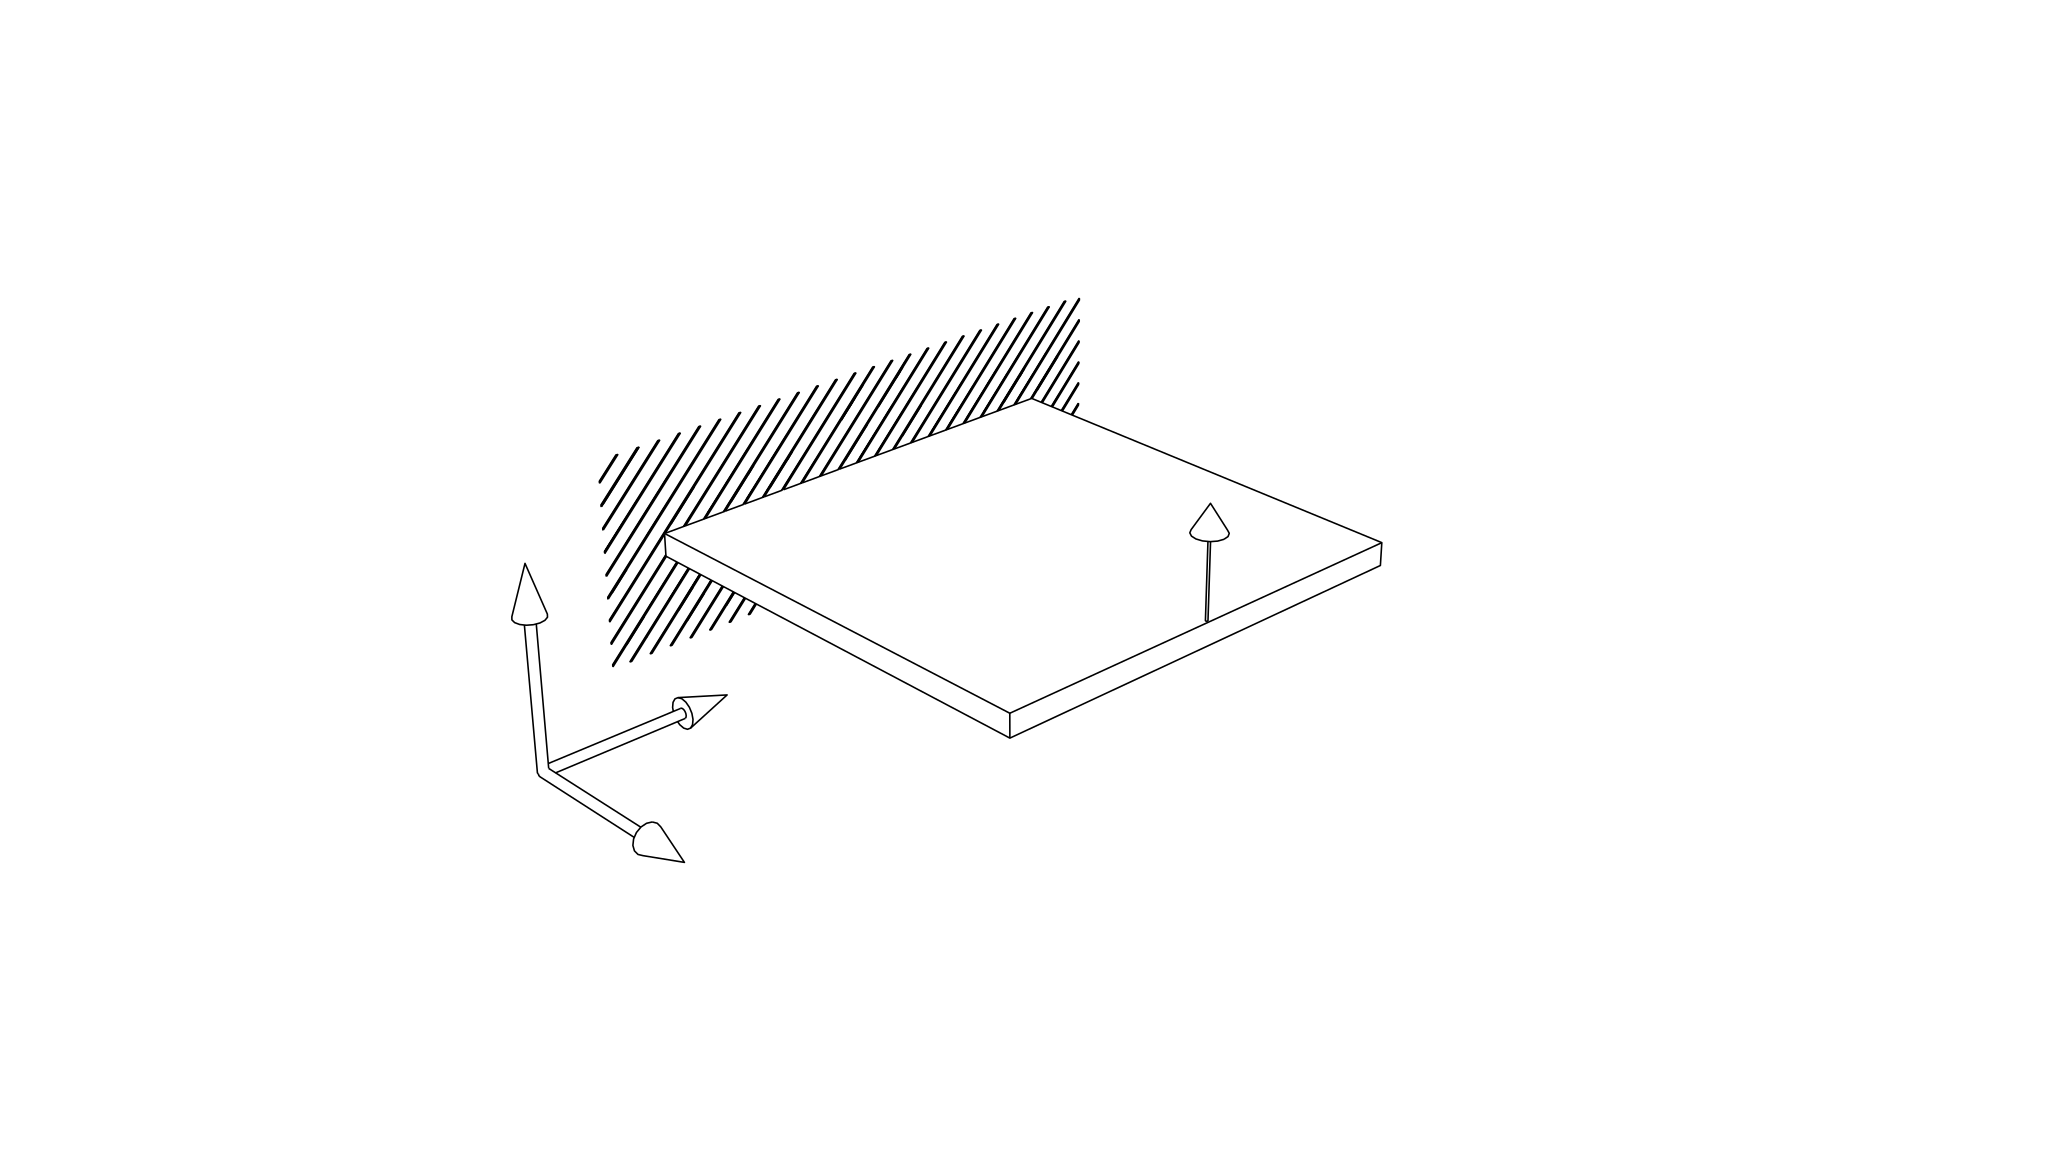
\includegraphics[width=0.4\linewidth]{\currfiledir/bended-plate.blend-min.svg.pdf}};

        \node[] at (-2.8,-2.2) {x};
        \node[] at (-2.0,-1.5) {y};
        \node[] at (-3.7,-0.0) {z};

        \node[rotate=+16] at (-2.4,+1.4) {fixed};

        \node[align=right] at (+0.8,+0.3) {Point A\\$F = \qty{10}{\kilo\newton}$};

        \node[] at (+0.6,-1.4) (A) {};
        \node[] at (+3.5,-0.0) (B) {};
        \node[] at (+1.0,+1.0) (C) {};
        \Dimline[($(A)+(+0.1,-0.1)$)][($(B)+(+0.1,-0.1)$)][below right][\qty{2}{\metre}];
        \Dimline[($(C)+(-0.2,+0.6)$)][($(B)+(+0.1,+0.5)$)][above right][\qty{2}{\metre}];
        \Dimline[($(B)+(+0.5,+0.1)$)][($(B)+(+0.5,+0.3)$)][right][\qty{0.1}{\metre}];

    \end{tikzpicture}
    \caption{Setup of the bended plate test}
    \label{bended-plate:fig:setup}
\end{figure}

\section{Analytical solution}
\label{bended-plate:sec:analytical-solution}

Neglecting geometrical non-linearity, the well-known analytical solution for
the deflection is given in \autoref{bended-plate:analytical-solution}.

\begin{equation}
    \label{bended-plate:analytical-solution}
    u_z = F \cdot \frac{a ^ 3}{3EI} = \qty{0.16}{\metre}
\end{equation}

\begin{samepage}
    with:
    \begin{description}
        \item[$u_{z}$] vertical deflection at the point load to be estimated.
        \item[$F$] point load (\qty{10}{\kilo\newton})
        \item[$a$] size of the plate (\qty{2}{\metre})
        \item[$E$] Young's modulus (\qty[per-mode = symbol]{1E6}{\kilo\newton\per\square\metre}; see \autoref{bended-plate:material-parameters})
        \item[$I$] Second moment of area, for this geometry $I = \frac{b \cdot t^3}{12} = \frac{\qty{2}{\metre} \cdot (\qty{0.1}{\metre})^3}{12} = 0.0001\overline{6} \qty{}{\metre}^4 $
    \end{description}
\end{samepage}

\section{Moose}
\label{bended-plate:sec:moose}

For this purely linear-elastic problem, the ‘NEWTON’ solver is used. The Moose
input files for this model and the corresponding MSH files are attached to this
document as a ZIP by the name of ‘bended-plate.i.zip’.

\fileattachment{\currfiledir/bended-plate.i.zip}{bended-plate.i.zip}

\section{Plaxis 3D}
\label{bended-plate:sec:plaxis3D}

The Plaxis command files for this model are attached to this document as a ZIP
by the name of ‘bended-plate.p3dlog.zip’.

\fileattachment{\currfiledir/bended-plate.p3dlog.zip}{bended-plate.p3dlog.zip}

\section{Results}
\label{bended-plate:sec:results}

The Moose and Plaxis models of this appendix use identical discretizations and
can therefore compared directly. In fact, the MSH files have been created by
exporting the Plaxis discretization. \autoref{bended-plate:tab:results} shows
element count, node count, and deflection of point ‘A’ for the models using
shell elements (TRI6) and volume elements (TET10) for different degrees of
discretization refinement.

\begin{figure}[htbp]
    \centering
    \begin{tikzpicture}

        \node[inner sep=0pt] (tri6) at (-4.5,0) {\includegraphics[width=0.45\linewidth]{\currfiledir/bended-plate-tri6-comp.png}};

        \node[inner sep=0pt] (tet10) at (+4.5,0) {\includegraphics[width=0.45\linewidth]{\currfiledir/bended-plate-tet10-comp.png}};

        \node[rotate=+20] at (-7.9,+2.7) {\tiny\qty{    44}{} TRI6};
        \node[rotate=+22] at (-7.8,+1.3) {\tiny\qty{   254}{} TRI6};
        \node[rotate=+28] at (-7.7,+0.0) {\tiny\qty{  3790}{} TRI6};
        \node[rotate=+31] at (-7.6,-1.2) {\tiny\qty{ 23446}{} TRI6};

        \node[rotate=+22] at (+1.1,+2.2) {\tiny\qty{   462}{} TET10};
        \node[rotate=+25] at (+1.2,+0.8) {\tiny\qty{  3516}{} TET10};
        \node[rotate=+34] at (+0.9,-0.8) {\tiny\qty{107819}{} TET10};

    \end{tikzpicture}
    \caption{Discretization of the bended plate models (grey: initial; colored: deformed state)}
    \label{bended-plate:fig:discretization}
\end{figure}

\begin{table}[htbp]
    \centering
    \caption{Resulting deflection for selected Plaxis models (geometrical non-linearity neglected)}
    \label{bended-plate:tab:results}
    \begin{tabularx}{\textwidth}{
            >{\hsize=0.2\hsize\linewidth=\hsize}X
            >{\hsize=0.2\hsize\linewidth=\hsize}R
            >{\hsize=0.2\hsize\linewidth=\hsize}R
            >{\hsize=0.2\hsize\linewidth=\hsize}Y
            >{\hsize=0.2\hsize\linewidth=\hsize}Y}

        \hline

        %& CPU-count / wall time (\si{\second}) & RAM (MB)                                                                                             

        Element & Element        & Node           & \multicolumn{2}{c}{Deflection of Point ‘A’
        (\si{\metre})}                                                                                                \\

        Type    & Count          & Count          & Moose                                      & Plaxis               \\

        \hline

        TRI6    & \qty{44}{}     & \qty{464}{}    & \qty{0.1646}{\metre}                       & \qty{0.1719}{\metre}
        \\

        TRI6    & \qty{254}{}    & \qty{2364}{}   & \qty{0.1696}{\metre}                       & \qty{0.1712}{\metre}
        \\ % \qty{63}{\mega\byte}

        TRI6    & \qty{3790}{}   & \qty{34850}{}  & \qty{0.1703}{\metre}                       &
        \qty{0.1715}{\metre}                                                                                          \\ % \qty{276}{\mega\byte}

        TRI6    & \qty{23446}{}  & \qty{233452}{} & \qty{0.1704}{\metre}                       &
        \qty{0.1716}{\metre}                                                                                          \\ % \qty{1480}{\mega\byte}

        \hline

        TET10   & \qty{462}{}    & \qty{1013}{}   & \qty{0.1565}{\metre}                       &
        \qty{0.1565}{\metre}                                                                                          \\

        TET10   & \qty{3516}{}   & \qty{3516}{}   & \qty{0.1587}{\metre}                       &
        \qty{0.1587}{\metre}                                                                                          \\

        TET10   & \qty{107819}{} & \qty{158749}{} & \qty{0.1599}{\metre}                       &
        \qty{0.1599}{\metre}                                                                                          \\

        \hline
    \end{tabularx}
\end{table}

\chapter{Bi-axial Shear Test}
\label{app:bi-axial-shear}
\section{Problem statement}

A bi-axial shear test of a homogenous material block of $\SI{1}{\metre} \times
    \SI{1}{\metre} \times \SI{1}{\metre}$ should be modeled to test the limit load
resulting from the Mohr-Coulomb failure criterion. The test setup is shown in
\autoref{bi-axial-shear-mohr-coulomb::fig:setup}. At xmin, ymin, ymax, and zmin
the block is fixed perpendicular to the face. The face xmax is loaded with a
constant (normal) pressure of $\sigma'_2 =
    \qty{1}{\kilo\newton\per\square\metre}$. The (normal) pressure $\sigma'_1$ at
zmax ramps up till no convergence can be found anymore. Material parameters are
givin in \autoref{bi-axial-shear-mohr-coulomb:material-parameters}.

\begin{table}[htbp]
    \centering
    \caption{Material parameters}
    \label{bi-axial-shear-mohr-coulomb:material-parameters}
    \begin{tabularx}{\textwidth}{XYY}

        \hline

        Property                        & Physical unit                                         & Value       \\

        \hline

        Youngs modulus $E$              & \si[per-mode = symbol]{\kilo\newton\per\square\metre} &
        \SI{1000}{}                                                                                           \\

        Poisson's ratio $\nu$           & -                                                     & \SI{0.25}{} \\

        Angle of inner friction $\phi'$ & \si[per-mode = symbol]{\degree}                       & \SI{30}{}
        \\

        Cohesion $c'$                   & \si[per-mode = symbol]{\kilo\newton\per\square\metre} & 1           \\

        \hline
    \end{tabularx}
\end{table}

\begin{figure}[htbp]
    \centering
    \begin{tikzpicture}

        % this image has been generated using Blender writing a SVG
        % using the "Freestyle SVG Exporter". The SVG is minimized
        % using third-party tools and finally converted to PDF using
        % Inkscape.
        \node[inner sep=0pt] (ch-stresses) at (0,0) {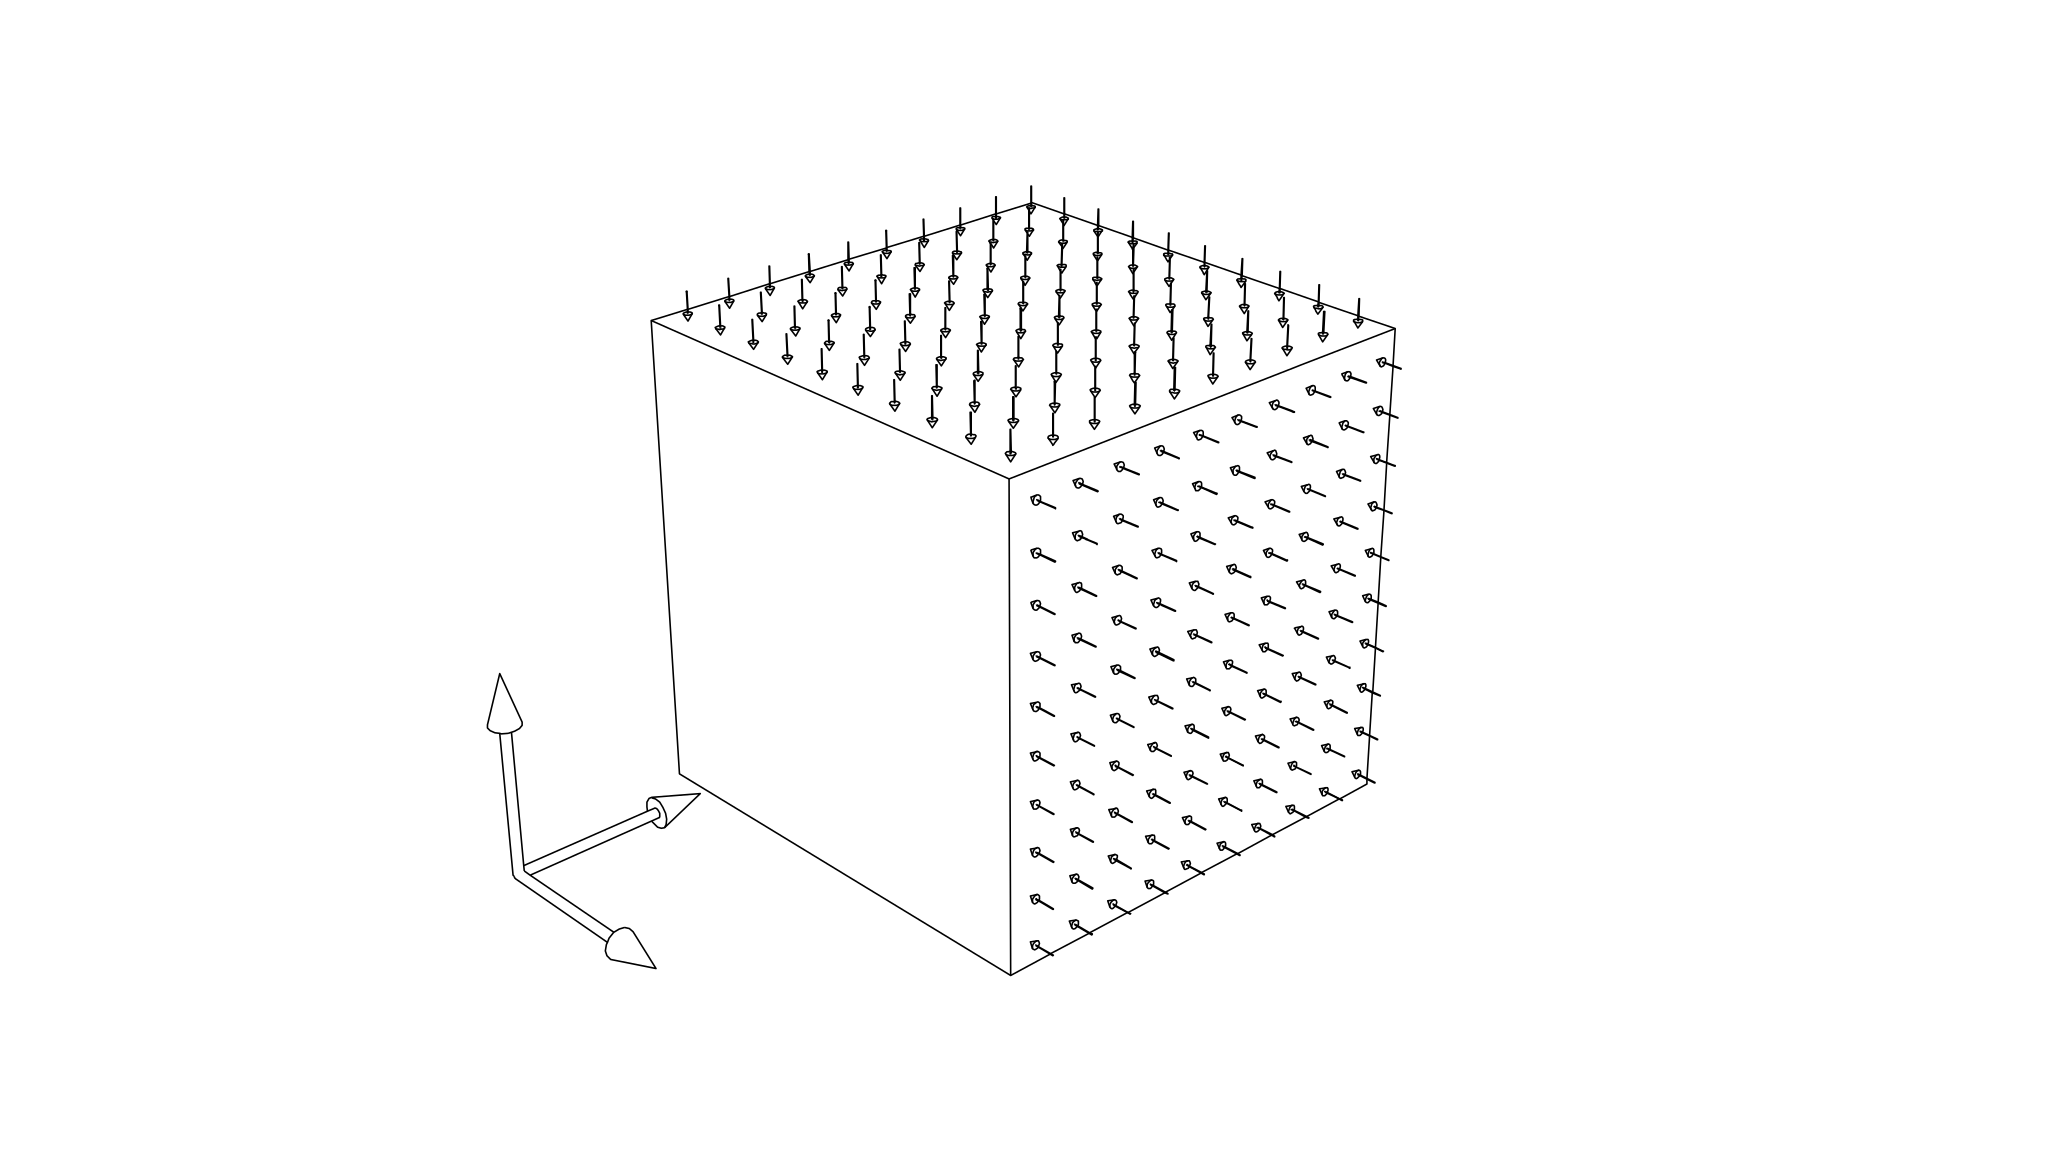
\includegraphics[width=0.4\linewidth]{\currfiledir/bi-axial-shear.blend.svg.pdf}};

        \node[] at (-3.0,-2.9) {x};
        \node[] at (-2.5,-1.5) {y};
        \node[] at (-3.0,-1.0) {z};

        \node[draw,circle,fill=white,minimum size=.5cm,inner sep=0pt, text width=1.5cm, align=center] (xmin_text) at (-4.0,+2.7) {xmin: $u_x \equiv 0$};
        \node (xmin) at (-2.1,+1.2) {};
        \path[->] (xmin_text) edge [out=0, in=180] (xmin);

        \node[draw,circle,fill=white,minimum size=.5cm,inner sep=0pt, text width=2.0cm, align=center] (xmax_text) at (+4.5,-2.5) {xmax: \\ $\sigma'_2 \equiv \qty[per-mode = fraction]{1}{\kilo\newton\per\square\metre} $};
        \node (xmax) at (+2.2,-1.4) {};
        \path[->] (xmax_text) edge [out=180, in=0] (xmax);

        \node[draw,circle,fill=white,minimum size=.5cm,inner sep=0pt, text width=1.5cm, align=center] (ymin_text) at (-3.8,+0.5) {ymin: $u_y \equiv 0$};
        \node (ymin) at (-0.8,-0.7) {};
        \path[->] (ymin_text) edge [out=0, in=180] (ymin);

        \node[draw,circle,fill=white,minimum size=.5cm,inner sep=0pt, text width=1.5cm, align=center] (ymax_text) at (+4.8,+1.7) {ymax: $u_y \equiv 0$};
        \node (ymax) at (+3.3,+0.0) {};
        \path[->] (ymax_text) edge [out=270, in=20] (ymax);

        \node[draw,circle,fill=white,minimum size=.5cm,inner sep=0pt, text width=1.5cm, align=center] (zmin_text) at (-1.2,-3.5) {zmin: $u_z \equiv 0$};
        \node (zmin) at (+0.2,-2.8) {};
        \path[->] (zmin_text) edge [out=0, in=270] (zmin);

        \node[draw,circle,fill=white,minimum size=.5cm,inner sep=0pt, text width=1.2cm, align=center] (zmax_text) at (+2.4,+3.2) {zmax: $\sigma'_1 = ?$};
        \node (zmax) at (+0.4,+1.7) {};
        \path[->] (zmax_text) edge [out=180, in=90] (zmax);

    \end{tikzpicture}
    \caption{Setup of the bi-axial shear test}
    \label{bi-axial-shear-mohr-coulomb::fig:setup}
\end{figure}

\section{Analytical solution}

From the yield function of the Mohr-Coulomb failure criterion shown in
\autoref{eqn:Mohr-Coulomb-failure-criterion} the limit load of the bi-axial
test can be derived as given in \autoref{eqn:bi-axial-test-limit-load}.

\begin{equation}
    \label{eqn:Mohr-Coulomb-failure-criterion}
    f = \frac{\abs{\sigma'_1 - \sigma'_2}}{2} + \frac{\sigma'_1 + \sigma'_2}{2} \cdot \sin{\phi'} - c' \cdot \cos{\phi'} = 0
\end{equation}

\begin{equation}
    \label{eqn:bi-axial-test-limit-load}
    \sigma'_1 = \sigma'_2 \cdot \frac{1 + \sin{\phi'}}{1 - \sin{\phi'}} - 2c' \cdot \frac{\cos{\phi'}}{1 - \sin{\phi'}}
    \approx \qty{-6.464}{\kilo\newton\per\square\metre}
\end{equation}

\section{Moose}

In the corresponding Moose model of this quasi-static problem a discretisation
of \qty{5184}{} TET10 elements and a transient executioner is used. The
linear-elastic material behaviour is modelled with a materials block of type of
\codeword{ComputeIsotropicElasticityTensor}. The ideal-plastic behaviour is
introduced with a materials block of type
\codeword{CappedMohrCoulombStressUpdate}. To avoid the cap of this materials
block to influence the system response, a very high tensile and compressive
strength is used.

The load $\sigma'_1$ ramps up linearly with time so that at $t =
    \qty{6.464}{\second}$ the load is $\sigma'_1 =
    \qty{-6.464}{\kilo\newton\per\square\metre}$. Due to the ideal-plastic nature
of the material behaviour, Moose will attempt to calculate time steps and
iteratively reduce the time step if convergence is not achieved. Eventually the
last converged time step should be at $t \approx \qty{6.464}{\second}$.

This model was calculated using the ‘PJFNK’ solver. The time step is initially
chosen to be \qty{0.25}{\second} and the minimum time step is limited to
\qty{0.001}{\second}. Due to the automatic cut-back of the time steps close to
failure, the last converged time step is at $t=\qty{6.43945}{\second}$. The
Moose input file for this model is attached to this document by the name of
‘bi-axial-shear.i’.

\fileattachment{\currfiledir/bi-axial-shear.i}{bi-axial-shear.i}

\section{Plaxis 3D}

The mesh used for Plaxis3D consists of 5130 TET10 elements.

\end{document}